\subsection{Robot description}

This section presents the kinematic model of the CLIO robot (see Fig. \ref{fig:3dmodel}). 
We model the robot as a fixed base manipulator with $n=9$ \gls{dofs} represented by the configuration vector $q \in \Rnum^n$. 
In the specific, we employ 2 \textit{passive} 
(rotational) joints to represent the attachment between the anchor point (a fixed link) and the rope.
The rope is modeled as an \textit{actuated} prismatic joint ($q_{R}$, followed by other 3 \textit{passive} rotational joints  to model 
the connection between the rope and the \textit{base link} of the robot 
\footnote{It would be equivalent to locate 3 joints	 at the anchor point and 2 at the base, 
	to avoid redundancy in the representation, it is necessary  to have only one passive joint along the rope axis.}. 
The propulsion mechanism that allows the robot to jump
is represented by a 3 \gls{dofs} robotic leg with a point-like foot that enables to exert a pure Cartesian force (no moment) on the wall. 
The leg has two \textit{subsequent} rotational joints, called  hip pitch ($q_{HP}$) and hip 
roll ($q_{HR}$) about the Y axis (green) and the X axis (red), respectively. The joints are useful to align  the leg in the 
direction of thrust impulse in order to avoid to generate centroidal moments that would initiate the pivoting of the robot around the Z axis (blue).
Finally a prismatic knee (($q_{K}$) joint is used to generate the \textit{thrusting} impulse. 
We built a Gazebo simulator based on the URDF  description of the robot.
\footnote{With the actual design the robot will not be able to stabilize itself on the wall, 
	however the design of a landing and stabilization mechanism is out of the scope of this work
	where we focus mainly on the jump motion, and will be addressed in future works. }

\begin{figure}
	\centering
	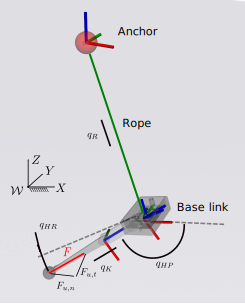
\includegraphics[width=0.8\columnwidth]{figs/3dmodel.pdf}
	\caption{Kinematics of the model of the robot.}
	\label{fig:3dmodel}
\end{figure}

The full dynamic equation with n-joint can be generalized into the following matrix form:  

\begin{align}
M (q) \ddot{q} + h(q,\dot{q}) = \mat{0_{5 \times 1} \\ \tau_a} + J^T F 
\end{align}

where $M \in \Rnum^{n \times n}$ is the inertia matrix; $h \in \Rnum^n$ represents the bias terms (Centrifugal, Coriolis and Gravity); and 
$J \in \Rnum^{3 \times n} $ is the Jacobian relative to the contact point mapping the contact force $F \in \Rnum^3$. 
Unless specified all the vectors are expressed in an inertial $\mathcal{W}$ frame. 
The under-actuation is captured by the vector $0_{5 \times 1}$ while 
the efforts of the actuated joints are grouped in the vector $\tau_a \in \Rnum^4$.

\subsection{Simplified Model}
We can define a simplified mathematical model by making the following assumptions: 1. The mass is entirely concentrated in the body attached to the wire, 2. We can unwind and rewind the wire but it is rigid and remains completely elongated (i.e., it cannot make bends), 3. The rewinder can pull the wire when winding it but cannot push it (i.e., it can only act as a brake during the unwinding phase).
A geometric sketch of the system is shown in Figure \ref{fig:sp}. where the polar angle is $\theta$ [rad], the Azimuth angle is $\phi$ [rad], and $l$ [m] is the length of the rigid rope. 

\begin{figure}
\includegraphics[width=\columnwidth]{figs/spherical_pendulum}
\caption{Logical scheme for the simplified model}
\label{fig:sp}
\end{figure}
Our input variables to the system are: 1. the rewinder pull action or
braking action $\mathbf{F}_r$ oriented along the wire, 2. an impulsive
push force $\mathbf{F}_u$ that the robot can generate when it is
attached to the mountain wall. 

Let $e$ be a frame attached to the weight $m$ 
with axis oriented along the $x$ axis, and let $w$ be the world
frame attached to the suspension point of the pendulum.  If we
consider the homogeneous transformation linking $e$ to $w$, we can
write
	\[
	T_e^w = \begin{bmatrix} R_z(\phi) &\begin{matrix}0\\0\\0 \end{matrix}  \\ \begin{matrix} 0 &0 &0 \end{matrix} & 1\end{bmatrix}  \begin{bmatrix} R_y(\pi/2 - \theta) &\begin{matrix}0\\0\\0 \end{matrix}  \\ \begin{matrix} 0 &0 &0 \end{matrix} & 1\end{bmatrix}  \begin{bmatrix} I_{3,3} &\begin{matrix}0\\0\\0 \end{matrix}  \\ \begin{matrix} L &0 &0 \end{matrix} & 1\end{bmatrix}  
	\]
where $R_z(\phi)$ is the rotation matrix of $\phi$ around $z$ , and $R_y(\alpha)$ is the rotation matrix of $\alpha$ around $y$. 
Simplifying $T_e^w$, gives 
	\[
	T_e^w = \begin{bmatrix} c_\phi s_\theta & -s_\phi & c_\phi c_\theta & l c_\phi s_\theta\\
		s_\phi s_\theta & c_\phi & c_\theta s_\phi & l s_\phi s_\theta\\
		-c_\theta & 0 & s_\theta &-l c_\theta\\
		0 & 0 &0 &1\end{bmatrix} 
	\]		
where $c_x$ is a shorthand for $\cos x$ , and $s_x$ is a shorthand for $\sin x$.
The position $\mathbf{p}$ of the mass can be extracted from the transformation matrix $T_e^w$ as : 
	\begin{align}  
		\mathbf{p} = \begin{bmatrix} x\\ y\\ z \end{bmatrix} =
		\begin{bmatrix}   
            l s_\theta c_\phi\\
			l s_\theta s_\phi\\
			-l c_\theta \end{bmatrix} \label{eq1}
    \end{align}
%From equation \ref{eq1}, we can compute the velocities and the kinetic energy:   
From equation \eqref{eq1}, the velocities along Cartesian axes are 
\begin{align*}
	\dot{x} &= 
	l c_\theta c_\phi \dot{\theta} - l s_\theta s_\phi \dot{\phi} + s_\theta c_\phi \dot{l} \\
	\dot{y} &= l c_\theta s_\phi \dot{\theta} + l s_\theta c_\phi \dot{\phi} + s_\theta s_\phi \dot{l} \\
	\dot{z} &= l s_\theta  \dot{\theta} - c_\theta \dot{l} 
\end{align*}
Next, the velocity of the mass squared
\begin{align*}
	v^2 &= \dot{x}^2 + \dot{y}^2 + \dot{z}^2 =  l^2 \dot{\theta}^2 + l^2 s_\theta^2 \dot{\phi}^2 + \dot{l}^2 		
%	&=  l^2 \dot{\theta}^2 + l^2 s_\theta^2 \dot{\phi}^2 + \dot{l}^2\\
\end{align*}
Thus, the kinetic energy $T$ and potential energy $V$  
\begin{align*}
	T &=\frac{ m }{2} v^2 =  \frac{m}{2} l^2 \left(\dot{\theta}^2 + s_\theta^2 \dot{\phi}^2 \right) + \frac{m }{2} \dot{l}^2  \\
    V &= mgz = -mgl c_\theta   \label{eq3}
\end{align*}
which leads to the Lagrangian function described as
\begin{equation}
	L = T - V = \frac{m}{2} l^2 \left(\dot{\theta}^2 + s_\theta^2 \dot{\phi}^2\right) + \frac{m}{2}\dot{l}^2 + mgl c_\theta
\end{equation}
The dynamics of the system will be obtained using the Euler-Lagrange equation:
\[
\frac{d}{dt}\frac{\partial L}{\partial \dot{q}_i} - \frac{\partial L}{\partial q_i} = Q_i^p 
\]
where $Q_i^p$ is the generalized force: 
$Q_i^p = (\mathbf{F}_r + \mathbf{F}_u) \cdot \frac{\partial \mathbf{p}}{\partial q_i}$ , \\
$\mathbf{F}_r$ is oriented along the rope and $\mathbf{F}_u$ is generated so that it does not have any component along the rope:		
	\begin{equation}
	\begin{aligned}
		\mathbf{F}_r  &= F_r \begin{bmatrix}
			c_\phi s_\theta\\
			s_\phi s_\theta\\
			-c_\theta
		\end{bmatrix}^T = F_r \mathbf{f}_r \\	
		\mathbf{F}_u &= F_{u,t}\begin{bmatrix}
			-s_\phi\\
			c_\phi\\
			0
		\end{bmatrix}^T + F_{u,n} \begin{bmatrix}
			c_\phi c_\theta \\
			s_\phi c_\theta\\
			s_\theta
		\end{bmatrix}^T &= F_{u,t} \mathbf{f}_{u,t} + F_{u,n} \mathbf{f}_{u,n}    	 
	\end{aligned}
	\label{eq:forces}
	\end{equation}
	Let the generalized coordinates $q_i$ be chosen as $q_1 = \theta$, $q_2 = \phi$ and $q_3 = l$ . The corresponding velocities are 
	\begin{align*}
	\qquad	\frac{\partial \mathbf{p}}{\partial q_1} = \frac{\partial \mathbf{p}}{\partial \theta} &= \begin{bmatrix}
			l c_\phi c_\theta\\
			l s_\phi c_\theta\\
			l s_\theta
		\end{bmatrix},  \text{and} \quad 
		\frac{\partial \mathbf{p}}{\partial q_2} = \frac{\partial \mathbf{p}}{\partial \phi} &= \begin{bmatrix}
			- l s_\phi s_\theta\\
			l c_\phi s_\theta\\
			0
		\end{bmatrix}, \\
		\frac{\partial \mathbf{p}}{\partial q_3} = \frac{\partial \mathbf{p}}{\partial l} &= \begin{bmatrix}
			c_\phi s_\theta\\
			s_\phi s_\theta\\
			-c_\theta
		\end{bmatrix} .
	\end{align*}

	Hence,
\begin{align*}
	Q_1^p &= \left(\mathbf{F}_r + \mathbf{F}_u\right)   \frac{\partial \mathbf{p}}{\partial q_1} 
	%% 		&= F_r \mathbf{f}_r \cdot  \frac{\partial \mathbf{p}}{\partial \theta} + \\
	%% 		&+ F_{u,t} \mathbf{f}_{u,t} \cdot  \frac{\partial \mathbf{p}}{\partial \theta} + \\
	%% 		&+ F_{u,n} \mathbf{f}_{u,n} \cdot  \frac{\partial \mathbf{p}}{\partial \theta}  =  \\
	%% 		&= F_{u,n} \mathbf{f}_{u,n} \cdot  \frac{\partial \mathbf{p}}{\partial \theta} = \\
	= F_{u,n} l , \\
	% 	\end{align*}
% 	\begin{align*}
	Q_2^p &= \left(\mathbf{F}_r + \mathbf{F}_u\right)   \frac{\partial \mathbf{p}}{\partial q_2}
	%% 		&= F_r \mathbf{f}_r \cdot  \frac{\partial \mathbf{p}}{\partial \phi} + \\
	%% 		&+ F_{u,t} \mathbf{f}_{u,t} \cdot  \frac{\partial \mathbf{p}}{\partial \phi} + \\
	%% 		&+ F_{u,n} \mathbf{f}_{u,n} \cdot  \frac{\partial \mathbf{p}}{\partial \phi}   = \\
	%% 		&= F_{u,t} \mathbf{f}_{u,t} \cdot  \frac{\partial \mathbf{p}}{\partial \phi} =\\
	= F_{u,t} l s_\theta,\\
	%% 	\end{align*}
%% 	\begin{align*}
	Q_3^p &= \left(\mathbf{F}_r + \mathbf{F}_u\right)   \frac{\partial \mathbf{p}}{\partial q_3}
	%% 		&= F_r \mathbf{f}_r \cdot  \frac{\partial \mathbf{p}}{\partial l} + \\
	%% 		&+ F_{u,t} \mathbf{f}_{u,t} \cdot  \frac{\partial \mathbf{p}}{\partial l} + \\
	%% 		&+ F_{u,n} \mathbf{f}_{u,n} \cdot  \frac{\partial \mathbf{p}}{\partial l}   = \\
	%% 		&= F_r \mathbf{f}_r \cdot  \frac{\partial \mathbf{p}}{\partial l} =\\
	= F_{r} .
\end{align*}
The Euler-Lagrange equations gives us, with the defined generalized coordinates: 
%% 	The first Euler-Lagrange equation yields
 	\begin{align*}
%		&\frac{d}{dt}\left(\frac{\partial L}{\partial \dot{\theta}} \right) - \frac{\partial L}{\partial \theta} = Q_1^p  \rightarrow  \\
%%		& \frac{d}{dt}\left(m l^2 \dot{\theta}\right) - (m l^2 s_\theta c_\theta \dot{\phi}^2 - m g l s_\theta) = F_{u,n}  l \\ 
 		  &m l^2 \ddot{\theta} + 2 m l \dot{\theta} \dot{l} - m l^2 s_\theta c_\theta \dot{\phi}^2 + m g l s_\theta = F_{u,n} . l\\
%% 		& \ddot{\theta} + \frac{2}{l} \dot{\theta} \dot{l} - c_\theta s_\theta \dot{\phi}^2 + \frac{g}{l}  s_\theta =  \frac{F_{u,n}  }{ml}    
%% 	\end{align*}
%% 	The second Euler-Lagrange equation yields
%% 	\begin{align*}
%% 		&\frac{d}{dt}\left(\frac{\partial L}{\partial \dot{\phi}} \right) - \frac{\partial L}{\partial \phi} = Q_2^p    \\
%% 		&\frac{d}{dt}\left(m l^2 s_\theta^2 \dot{\phi}\right) = F_{u,t}  l  s_\theta\\
 		 &\ddot{\phi} ml^2 s^2_\theta + 2 m l \dot{l} s_\theta^2 \dot{\phi} + 2 m l^2 s_\theta c_\theta \dot{\theta} \dot{\phi}  = F_{u,t}  l  s_\theta\\
%%		&\ddot{\phi} + 2 \frac{c_\theta}{s_\theta} \dot{\theta} \dot{\phi} + \frac{2}{l} \dot{\phi} \dot{l} = \frac{F_{u,t}}{ml s_\theta}
%% 	\end{align*}
%% 	The third Euler-Lagrange equation is as follows:
%% 	\begin{align*}
%% 		&\frac{d}{dt}\left(\frac{\partial L}{\partial \dot{l}} \right) - \frac{\partial L}{\partial l} = Q_3^p    \\
%% 		&\frac{d}{dt}\left(m\dot{l}\right) - (m l \dot{\theta}^2 + m l s^2_\theta \dot{\phi}^2 + m g c_\theta) = F_r ,
 		&m \ddot{l} - m l \dot{\theta}^2 - m l s^2_\theta \dot{\phi}^2 - m g c_\theta = F_r 
%% 		&\ddot{l} - l \dot{\theta}^2 - l s^2_\theta \dot{\phi}^2 - g c_\theta = \frac{F_r}{m} 
 	\end{align*}
           %%
        Overall, the non-linear dynamic equations of the system 
%        Overall, the nonlinear equations of the system are:
        \begin{equation}
        \begin{aligned}
		&\ddot{\theta} + \frac{2}{l} \dot{\theta} \dot{l} - c_\theta s_\theta  \dot{\phi}^2 + \frac{g}{l}  s_\theta =  \frac{1}{ml}F_{u,n} \\
		&\ddot{\phi} + 2 \frac{c_\theta}{s_\theta} \dot{\theta} \dot{\phi} + \frac{2}{l} \dot{\phi} \dot{l} = \frac{1}{ml s_\theta} F_{u,t} \\
		&\ddot{l} - l \dot{\theta}^2 - l s^2_\theta \dot{\phi}^2 - g c_\theta = \frac{1}{m} F_r .
	\end{aligned}
        \label{eq:nonlinearDyn}
        \end{equation}
        Clearly, in this derivation of the model, we have heavily
        relied on the point-mass nature of the body.  A possible issue
        could be the rotational dynamics of the body around its axis,
        which could waste energy generating unnecessary motions and
        impede the landing phase. This issue will be part of our
        future work. However, as discussed next, under reasonable
        assumptions (e.g., thrusting force oriented in the direction
        of the center of mass), the results based on the simplified
        model can be applied to a realistic system with a good approximation.

\subsection{Robot motion: problems and solution overview}
The problem of moving CLIO between two given configurations is not an
easy task.  First of all, even the simplified dynamics in
Equation~\eqref{eq:nonlinearDyn} is highly nonlinear.  Second, 
the configurations the robot moves between can be in general two 
distant points of the workspace. Therefore, it is not possible to
use the linearized dynamics.  Third, one of our
actuators, the thrusting force $\mathbf{F}_u$, has an impulsive nature
and operates at discrete time instants. Therefore, it is not possible
to use this part of the actuation in any feedback control scheme.
Finally, the way the tangential component $F_{u,t}$ is generated is by
using friction. Therefore, the two components $F_{u,n}$ and $F_{u,t}$ are linked
by a nonlinear constraints expressing the friction cone. Because the friction cone
depends on the specific point or area where the robot is pointing its leg,
this mechanism is not totally reliable (i.e., there can be significant deviation
between the generated and the exacted values of $F_{u,t}$).

In view of this complexity, we propose an approach based on two steps:
1. first a motion strategy is planned prior to starting the motion,
2. after the take of phase a motion controller operates on
$\mathbf{F}_r$ in a feedback control scheme to fix small deviation and
to secure that the robot lands close enough to the expected position.

